% \noindent \textcolor{red}{$\left[Typo\ correction\right]$}
% \noindent  \textcolor{red}{$\bullet$ Eq. (3) in the main paper should be corrected into 
% \begin{equation}\label{eq:sup_balancing}
% \hat{z}^{i}_{k} = z^{i}_{k} + \frac{c_{k}}{\max_{i=0}^{C-1}(c_{i})}|\delta(\sigma)|,\quad c_{k} =\log \frac{\sum_{j=0}^{C-1}q_{j}}{q_{k}}
% \end{equation}}
% \noindent  \textcolor{red}{$\bullet$ The ``Exploration on the variance $k$" in the ``Ablation Studies" section should be corrected into ``Exploration on the variance $\sigma$"} 


\definecolor{myblue}{RGB}{0,0,255}



\section{Overview}
In this supplementary material, we first provide more details for reproducibility in \cref{sec-sup:reprodu}.
%
We further explore a potential improvement of \method and corresponding preliminary results in \cref{sec-sup:more-expro}.
%
Then we demonstrate our \method with more UDA methods on both the \textit{GTA5 $\to$ Cityscapes} and \textit{SYNTHIA $\to$ Cityscapes} settings in \cref{sec-sup:comp-uda}.
%
Intuitive feature space visualization is demonstrated by t-SNE method in \cref{sec-sup:tsne-visual}.
%
Pseudo-code for direct understanding of \method is provided in \cref{sec-sup:pseudo-code}.
%
Information about computational overhead and distribution estimation is exhibited in \cref{sec-sup:training-time} and \cref{sec-sup:estimation-labeled}.




\section{More Details for Reproducibility}\label{sec-sup:reprodu}
\noindent \textbf{Details for parameters.}
As we mentioned in the paper, the only parameter for \method is the $\sigma$ in Eq. (\textcolor{red}{3}).

We set $\sigma=4$ for unsupervised domain adaptive semantic segmentation task under the \textit{SYNTHIA $\to$ Cityscapes} setting.
%
For all the other tasks, we set $\sigma=6$ consistently.
%
Besides, the $\delta(\sigma)$ term is clamped into $\left[0, 1\right]$ to avoid particularly large values that makes training unstable.




%
\noindent \textbf{Details for data augmentation.}
We follow DACS~\cite{tranheden2021dacs}, using color jitter, Gaussian blur, and ClassMix~\cite{classmix} as the augmentation selections.



\section{More Exploration of Variation} \label{sec-sup:more-expro}



We explore the improvement over \method.
%
We set the $\sigma$ in Eq. (\textcolor{red}{3}) as a temporal variable: $\sigma(t)$, where $t$ denotes current iteration, $t_{mid}$ and $\sigma_{0}$ are hyper-parameters with preset values.
%
\cref{fig:more_variation} depicts how $\sigma$ changes with iterations.

%
The main idea is to let the perturbation increase gradually before $t_{mid}$ to obtain an effective variation. 
%
After $t_{mid}$, we should let the variation decrease so that the model convergence is not affected.
%
This exploration is easy to implement. 
%
We conducted the experiment under \textit{GTA5 $\to$ Cityscapes} benchmark.
%
$t_{end}=40k$, $t_{mid}=30k$ and $\sigma_{0}=6$.

\begin{figure}[ht]
    \centering
    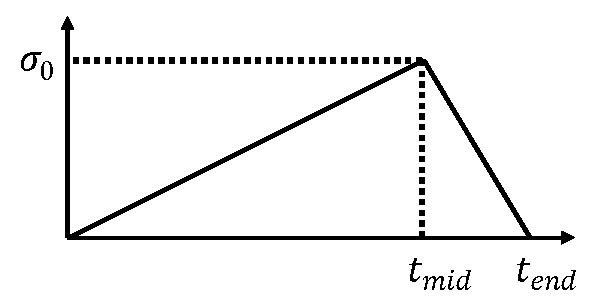
\includegraphics[width=1.0\linewidth]{figures/sup_variation.pdf}
    \vspace{-15pt}
    \caption{
        \textbf{$\sigma$ that changes with training iterations.}
        %
        $t_{end}$ is the total iterations.
        %
        $t_{mid}$ is the turning point of $\sigma$ with a corresponding maximum value $\sigma_{0}$.
    }
    \label{fig:more_variation}
    \vspace{-10pt}
\end{figure}

\begin{table}[!ht]
\centering
\caption{
%
\textbf{Exploration on temporal variation of \method.} ``+tv" denotes our proposed ``temporal variable".
%
}
\setlength{\tabcolsep}{16pt}
\label{tab:sup_explor}
\vspace{-8pt}
\begin{tabular}{ccc}
\toprule
 Baseline &  \method &  \textbf{\method+tv}  \\
\midrule
 68.3 &   69.6\textbf{\up{1.3}}        &    \textbf{70.0\up{1.7}}     \\
\bottomrule
\end{tabular}
\vspace{-10pt}
\end{table}

The result is demonstrated in ~\cref{tab:sup_explor}.
%
The baseline is DAFormer$\ddag$ model.
%
This table suggests that this ``temporal variable" does improve the original \method.
%
The overall result indicates that there is an opportunity to further improve our approach.



\section{More Comparisons on UDA Benchmark}  \label{sec-sup:comp-uda}
%
% Most studies use CNN as the backbone.
% %
% In this section, we also compare category performance of our method with other state-of-the-art CNN-based methods.
% %
% As shown in \cref{tab:sup-udaperformance}, our \method with ResNet-101 achieves competitive performance among existing methods.
% %
% Note that, we report the performances of ProDA \cite{zhang2021prototypical} and CPSL \cite{li2022class} in \cref{tab:sup-udaperformance} \textit{without} knowledge distillation (which uses self-supervised trained models) for a fair comparison.
% %
% On the SYNTHIA $\to$ Cityscapes benchmark, we set $\mu'=0.9999$ for our \method.
% As shown in \cref{tab:supsynthiaperformance}, our method also demonstrates competitive performance, which is slightly lower than CPSL, a class-balanced training approach that is orthogonal to our work.
%
%%%%%%%%%%%%%%%%%%%%%%%%%%%%%%%%%%%%%%%%%%%%%%%%%%%%%%%%%%%%%%%%%
\begin{table*}[t]
\centering
\caption{
Comparison with state-of-the-art alternatives on \textit{GTA5 $\to$ Cityscapes} benchmark with ResNet-101~\cite{he2016deep} and DeepLab-V2~\cite{deeplab}.
%
The results are averaged over 3 random seeds.
%
The top performance is highlighted in \textbf{bold} font and the second score is \textit{underlined}.}
\vspace{10pt}
\label{tab:supgta5performance}
\setlength{\tabcolsep}{2.3pt}
\scalebox{0.95}{
\begin{tabular}{l | ccccccccccccccccccc | cc}
\toprule
Method &
\rotatebox{90}{Road} & \rotatebox{90}{S.walk} & \rotatebox{90}{Build.} & \rotatebox{90}{Wall*} & \rotatebox{90}{Fence*} & \rotatebox{90}{Pole*} & \rotatebox{90}{T.light} & \rotatebox{90}{Sign} & \rotatebox{90}{Veget.} & \rotatebox{90}{Terrain} & \rotatebox{90}{Sky} & \rotatebox{90}{Person} & \rotatebox{90}{Rider} & \rotatebox{90}{Car} & \rotatebox{90}{Truck} & \rotatebox{90}{Bus} & \rotatebox{90}{Train} & \rotatebox{90}{M.bike} & \rotatebox{90}{Bike} & mIoU  \\
\midrule
source only & 70.2 & 14.6 & 71.3 & 24.1 & 15.3 & 25.5 & 32.1 & 13.5 & 82.9 & 25.1 & 78.0 & 56.2 & 33.3 & 76.3 & 26.6 & 29.8 & 12.3 & 28.5 & 18.0 & 38.6 \\
\midrule
AdaptSeg~\cite{tsai2018learning} & 86.5 & 36.0 & 79.9 & 23.4 & 23.3 & 23.9 & 35.2 & 14.8 & 83.4 & 33.3 & 75.6 & 58.5 & 27.6 & 73.7 & 32.5 & 35.4 & 3.9 & 30.1 & 28.1 & 41.4 \\
%
CyCADA~\cite{hoffman2018cycada} & 86.7 & 35.6 & 80.1 & 19.8 & 17.5 & 38.0 & 39.9 & 41.5 & 82.7 & 27.9 & 73.6 & 64.9 & 19.0 & 65.0 & 12.0 & 28.6 & 4.5 & 31.1 & 42.0 & 42.7 \\
%
ADVENT~\cite{vu2019advent} & 89.4 & 33.1 & 81.0 & 26.6 & 26.8 & 27.2 & 33.5 & 24.7 & 83.9 & 36.7 & 78.8 & 58.7 & 30.5 & 84.8 & 38.5 & 44.5 & 1.7 & 31.6 & 32.4 & 45.5 \\
%
CBST~\cite{zou2018unsupervised} & 91.8 & 53.5 & 80.5 & 32.7 & 21.0 & 34.0 & 28.9 & 20.4 & 83.9 & 34.2 & 80.9 & 53.1 & 24.0 & 82.7 & 30.3 & 35.9 & 16.0 & 25.9 & 42.8 & 45.9 \\
%
PCLA~\cite{kang2020pixel} & 84.0 & 30.4 & 82.4 & 35.3 & 24.8 & 32.2 & 36.8 & 24.5 & 85.5 & 37.2 & 78.6 & 66.9 & 32.8 & 85.5 & 40.4 & 48.0 & 8.8 & 29.8 & 41.8 & 47.7 \\
%
FADA~\cite{wang2020classes} & 92.5 & 47.5 & 85.1 & 37.6 & 32.8 & 33.4 & 33.8 & 18.4 & 85.3 & 37.7 & 83.5 & 63.2 & \underline{39.7} & 87.5 & 32.9 & 47.8 & 1.6 & 34.9 & 39.5 & 49.2 \\
%
MCS~\cite{chung2022maximizing} & 92.6 & 54.0 & 85.4 & 35.0 & 26.0 & 32.4 & 41.2 & 29.7 & 85.1 & 40.9 & 85.4 & 62.6 & 34.7 & 85.7 & 35.6 & 50.8 & 2.4 & 31.0 & 34.0 & 49.7 \\
%
CAG~\cite{zhang2019category} & 90.4 & 51.6 & 83.8 & 34.2 & 27.8 & 38.4 & 25.3 & 48.4 & 85.4 & 38.2 & 78.1 & 58.6 & 34.6 & 84.7 & 21.9 & 42.7 & \textbf{41.1} & 29.3 & 37.2 & 50.2 \\
%
FDA~\cite{yang2020fda} & 92.5 & 53.3 & 82.4 & 26.5 & 27.6 & 36.4 & 40.6 & 38.9 & 82.3 & 39.8 & 78.0 & 62.6 & 34.4 & 84.9 & 34.1 & 53.1 & 16.9 & 27.7 & 46.4 & 50.5 \\
%
PIT~\cite{lv2020cross} & 87.5 & 43.4 & 78.8 & 31.2 & 30.2 & 36.3 & 39.3 & 42.0 & 79.2 & 37.1 & 79.3 & 65.4 & 37.5 & 83.2 & \underline{46.0} & 45.6 & \underline{25.7} & 23.5 & 49.9 & 50.6 \\
%
IAST~\cite{mei2020instance} & \underline{93.8} & 57.8 & 85.1 & 39.5 & 26.7 & 26.2 & 43.1 & 34.7 & 84.9 & 32.9 & 88.0 & 62.6 & 29.0 & 87.3 & 39.2 & 49.6 & 23.2 & 34.7 & 39.6 & 51.5 \\
%
DACS~\cite{tranheden2021dacs} & 89.9 & 39.7 & \underline{87.9} & 30.7 & 39.5 & 38.5 & 46.4 & \underline{52.8} & \underline{88.0} & \textbf{44.0} & \underline{88.8} & 67.2 & 35.8 & 84.5 & 45.7 & 50.2 & 0.0 & 27.3 & 34.0 & 52.1 \\
%
RCCR~\cite{zhou2021domain} & 93.7 & \underline{60.4} & 86.5 & 41.1 & 32.0 & 37.3 & 38.7 & 38.6 & 87.2 & 43.0 & 85.5 & 65.4 & 35.1 & \underline{88.3} & 41.8 & 51.6 & 0.0 & 38.0 & 52.1 & 53.5 \\  
%
ProDA~\cite{zhang2021prototypical} & 91.5 & 52.4 & 82.9 & \underline{42.0} & \underline{35.7} & 40.0 & 44.4 & 43.3 & 87.0 & \underline{43.8} & 79.5 & 66.5 & 31.4 & 86.7 & 41.1 & 52.5 & 0.0 & \underline{45.4} & \underline{53.8} & 53.7 \\  
%
CPSL~\cite{li2022class} & 91.7 & 52.9 & 83.6 & \textbf{43.0} & 32.3 & \textbf{43.7} & \underline{51.3} & 42.8 & 85.4 & 37.6 & 81.1 & \textbf{69.5} & 30.0 & 88.1 & 44.1 & \textbf{59.9} & 24.9 & \textbf{47.2} & 48.4 & \underline{55.7} \\
%
\midrule
%
\method (ours) & \textbf{94.9} & \textbf{68.2} & \textbf{88.8} & 40.9 & \textbf{37.1} & \underline{42.6} & \textbf{52.1} & \textbf{62.1} & \textbf{88.3} & 43.3 & \textbf{89.3} & \underline{68.6} & \textbf{44.5} & \textbf{88.9} & \textbf{56.0} & \underline{54.6} & 3.8 & 38.6 & \textbf{58.3} & \textbf{59.0} \\
 %
\bottomrule
\end{tabular}}
\vspace{-5pt}
\end{table*}


\begin{table*}[t]
\centering
\caption{
Comparison with state-of-the-art alternatives on \textit{SYNTHIA $\to$ Cityscapes} benchmark with ResNet-101~\cite{he2016deep} and DeepLab-V2~\cite{deeplab}. 
%
The results are averaged over 3 random seeds.
%
The mIoU and the mIoU* indicate we compute mean IoU over 16 and 13 categories, respectively.
%
The top performance is highlighted in \textbf{bold} font and the second score is \textit{underlined}.}
\vspace{10pt}
\label{tab:supsynthiaperformance}
\setlength{\tabcolsep}{2.3pt}
\scalebox{1}{
\begin{tabular}{l | cccccccccccccccc | cc}
\toprule
Method &
\rotatebox{90}{Road} & \rotatebox{90}{S.walk} & \rotatebox{90}{Build.} & \rotatebox{90}{Wall*} & \rotatebox{90}{Fence*} & \rotatebox{90}{Pole*} & \rotatebox{90}{T.light} & \rotatebox{90}{Sign} & \rotatebox{90}{Veget.} & \rotatebox{90}{Sky} & \rotatebox{90}{Person} & \rotatebox{90}{Rider} & \rotatebox{90}{Car} & \rotatebox{90}{Bus} & \rotatebox{90}{M.bike} & \rotatebox{90}{Bike} & mIoU & mIoU* \\
\midrule
source only$^\dag$ & 55.6 & 23.8 & 74.6 & 9.2 & 0.2 & 24.4 & 6.1 & 12.1 & 74.8 & 79.0 & 55.3 & 19.1 & 39.6 & 23.3 & 13.7 & 25.0 & 33.5 & 38.6 \\
\midrule
AdaptSeg~\cite{tsai2018learning} & 79.2 & 37.2 & 78.8 & - & - & - & 9.9 & 10.5 & 78.2 & 80.5 & 53.5 & 19.6 & 67.0 & 29.5 & 21.6 & 31.3 & - & 45.9 \\
%
ADVENT~\cite{vu2019advent} & 85.6 & 42.2 & 79.7 & 8.7 & 0.4 & 25.9 & 5.4 & 8.1 & 80.4 & 84.1 & 57.9 & 23.8 & 73.3 & 36.4 & 14.2 & 33.0 & 41.2 & 48.0 \\
%
CBST~\cite{zou2018unsupervised} & 68.0 & 29.9 & 76.3 & 10.8 & 1.4 & 33.9 & 22.8 & 29.5 & 77.6 & 78.3 & 60.6 & 28.3 & 81.6 & 23.5 & 18.8 & 39.8 & 42.6 & 48.9 \\
%
CAG~\cite{zhang2019category} & 84.7 & 40.8 & 81.7 & 7.8 & 0.0 & 35.1 & 13.3 & 22.7 & 84.5 & 77.6 & 64.2 & 27.8 & 80.9 & 19.7 & 22.7 & 48.3 & 44.5 & 51.5\\
%
PIT~\cite{lv2020cross} & 83.1 & 27.6 & 81.5 & 8.9 & 0.3 & 21.8 & 26.4 & 33.8 & 76.4 & 78.8 & 64.2 & 27.6 & 79.6 & 31.2 & 31.0 & 31.3 & 44.0 & 51.8 \\
%
FDA~\cite{yang2020fda} & 79.3 & 35.0 & 73.2 & - & - & - & 19.9 & 24.0 & 61.7 & 82.6 & 61.4 & 31.1 & 83.9 & 40.8 & 38.4 & 51.1 & - & 52.5 \\
%
FADA~\cite{wang2020classes} & 84.5 & 40.1 & 83.1 & 4.8 & 0.0 & 34.3 & 20.1 & 27.2 & 84.8 & 84.0 & 53.5 & 22.6 & 85.4 & 43.7 & 26.8 & 27.8 & 45.2 & 52.5 \\
%
MCS~\cite{chung2022maximizing} & \underline{88.3} & \textbf{47.3} & 80.1 & - & - & - & 21.6 & 20.2 & 79.6 & 82.1 & 59.0 & 28.2 & 82.0 & 39.2 & 17.3 & 46.7 & - & 53.2 \\
%
PyCDA~\cite{lian2019constructing} & 75.5 & 30.9 & 83.3 & 20.8 & 0.7 & 32.7 & 27.3 & 33.5 & 84.7 & 85.0 & 64.1 & 25.4 & 85.0 & 45.2 & 21.2 & 32.0 & 46.7 & 53.3 \\
%
PLCA~\cite{kang2020pixel} & 82.6 & 29.0 & 81.0 & 11.2 & 0.2 & 33.6 & 24.9 & 18.3 & 82.8 & 82.3 & 62.1 & 26.5 & 85.6 & 48.9 & 26.8 & 52.2 & 46.8 & 54.0 \\
%
DACS~\cite{tranheden2021dacs} & 80.6 & 25.1 & 81.9 & 21.5 & 2.9 & 37.2 & 22.7 & 24.0 & 83.7 & \textbf{90.8} & 67.6 & \underline{38.3} & 82.9 & 38.9 & 28.5 & 47.6 & 48.3 & 54.8 \\
%
RCCR~\cite{zhou2021domain} & 79.4 & 45.3 & 83.3 & - & - & - & 24.7 & 29.6 & 68.9 & 87.5 & 63.1 & 33.8 & 87.0 & 51.0 & 32.1 & 52.1 & - & 56.8 \\
%
IAST~\cite{mei2020instance} & 81.9 & 41.5 & 83.3 & 17.7 & \underline{4.6} & 32.3 & 30.9 & 28.8 & 83.4 & 85.0 & 65.5 & 30.8 & 86.5 & 38.2 & 33.1 & 52.7 & 49.8 & 57.0 \\
%
ProDA~\cite{zhang2021prototypical} & 87.1 & 44.0 & 83.2 & \textbf{26.9} & 0.7 & 42.0 & 45.8 & \underline{34.2} & 86.7 & 81.3 & 68.4 & 22.1 & \underline{87.7} & 50.0 & 31.4 & 38.6 & 51.9 & 58.5 \\
%
SAC~\cite{araslanov2021self} & \textbf{89.3} & \underline{47.2} & \underline{85.5} & \underline{26.5} & 1.3 & \textbf{43.0} & 45.5 & 32.0 & \textbf{87.1} & \underline{89.3} & 63.6 & 25.4 & 86.9 & 35.6 & 30.4 & 53.0 & 52.6 & 59.3 \\
%
CPSL~\cite{li2022class} & 87.3 & 44.4 & 83.8 & 25.0 & 0.4 & \underline{42.9} & \underline{47.5} & 32.4 & 86.5 & 83.3 & \underline{69.6} & 29.1 & \textbf{89.4} & \textbf{52.1} & \underline{42.6} & \underline{54.1} & \underline{54.4} & \underline{61.7} \\ 
%
\midrule
%
\method (ours) &
70.4	&28.9&	\textbf{89.2}&	25.2&	\textbf{19.9}&	40.2&	\textbf{55.2}&	\textbf{50.3}&	\underline{86.9}&	84.2&	\textbf{76.4}&	\textbf{40.5}&	79.6&	\underline{51.3}&	\textbf{49.2}&	\textbf{61.2}&	\textbf{56.8}& \textbf{63.3}\\ 
 %
\bottomrule
\end{tabular}}
\vspace{-5pt}
\end{table*}



We add more comparisons of \method with previous UDA methods for GTA5 $\to$ Cityscapes in
\cref{tab:supgta5performance} and for SYNTHIA $\to$ Cityscapes in \cref{tab:supsynthiaperformance}.
%

We include following methods for comparision: AdaptSeg~\cite{tsai2018learning}, CyCADA~\cite{hoffman2018cycada},  ADVENT~\cite{vu2019advent}, FADA~\cite{wang2020classes}, CBST~\cite{zou2018unsupervised}, IAST~\cite{mei2020instance}, CAG~\cite{zhang2019category}, ProDA~\cite{zhang2021prototypical}, SAC~\cite{araslanov2021self}, CPSL~\cite{li2022class},
PLCA~\cite{kang2020pixel}, RCCR~\cite{zhou2021domain}, and MCS~\cite{chung2022maximizing}.
%
All methods in \cref{tab:supgta5performance} and \cref{tab:supsynthiaperformance} are based on ResNet-101~\cite{he2016deep} + DeepLab V2~\cite{deeplab}.
%


\method surpasses other alternatives by a large margin, achieving mIoU of $59.0\%$ on \textit{GTA5 $\to$ Cityscapes}, and $56.8\%$ over 16 classes and $63.3\%$ over 13 classes on \textit{SYNTHIA $\to$ Cityscapes}, respectively.
%





\section{Visualization on Feature Space} \label{sec-sup:tsne-visual}
We use t-SNE~\cite{van2008visualizing} to visualize the logit feature space in ~\cref{fig:tsne-visual}.
%
In terms of the degree of confusion in the feature space, \method improves the baseline and proves its superiority.


\section{Pseudo-code} \label{sec-sup:pseudo-code}
To make \method easy to understand, we provide pseudo-code in a Pytorch-like style in \cref{alg:code}.
%
% algorithm
\begin{algorithm}[ht]
    \caption{Pseudo-code of \method in a PyTorch-like style.}
    \label{alg:code}
    \definecolor{codeblue}{rgb}{0.25,0.5,0.5}
    \lstset{
      backgroundcolor=\color{white},
      basicstyle=\fontsize{7.2pt}{7.2pt}\ttfamily\selectfont,
      columns=fullflexible,
      breaklines=true,
      captionpos=b,
      commentstyle=\fontsize{7.2pt}{7.2pt}\color{codeblue},
      keywordstyle=\fontsize{7.2pt}{7.2pt},
    %  frame=tb,
    }
    \begin{lstlisting}[language=python]
# frequency_list: a list containing the frequency of pixels of each category.
# pred: model output logits
# target: ground-truch label
# sigma: hyper-paramter

def BLV_Loss(pred, target, sigma, frequency_list):

    
    sampler = torch.distributions.normal.Normal(0, sigma)

    noise = sampler.sample(pred.shape).clamp(0, 1).to(pred.device)

    pred = pred + (noise.abs().permute(0, 2, 3, 1) * frequency_list / frequency_list.max()).permute(0, 3, 1, 2)

    loss = torch.nn.functional.cross_entropy(pred, target)

    return loss

\end{lstlisting}
\end{algorithm}

\begin{figure}[ht]
    \centering
    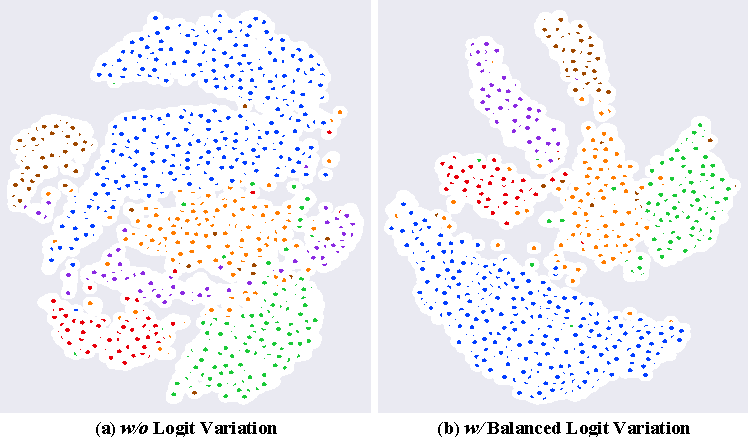
\includegraphics[width=1.0\linewidth]{figures/sup_tsne.pdf}
    \vspace{-15pt}
    \caption{
        \textbf{t-SNE visualization from the logit feature space.}
        (a) Without logit variation, the spacing between instances of different categories is small, resulting in easy misclassification.
        %
        (b) With balanced logit variation, instances are easier to distinguish.
    }
    \label{fig:tsne-visual}
    \vspace{-10pt}
\end{figure}




\section{Computational Overhead} \label{sec-sup:training-time}

We list parts of training time comparison in \cref{tab:training_time}, which suggests the computational overhead introduced by \method is limited and has a trivial impact on the overall training time.
%
As a plug-in design, \method demonstrates its superiority.

\vspace{-5pt}
\begin{table}[!ht]
\centering
\caption{
Training time comparison (with 8 V100 GPUs).
}
\label{tab:training_time}
\vspace{-10pt}
\setlength{\tabcolsep}{10pt}
\scalebox{0.85}{
\begin{tabular}{cc|cc}
\toprule
Backbone & Decoder & \textit{w/o} \method & \textit{w/} \method \\
\midrule
HRNet-18 & OCRHead & 20h11m & 21h07m (+4.6\%)\\
\midrule 
ResNet50&UperHead & 16h20m &16h47m (+2.8\%)\\
\bottomrule
\end{tabular}}
\vspace{-10pt}
\end{table}







\section{Estimation from the Labeled Data} \label{sec-sup:estimation-labeled}

Under semi-supervised settings, we have tried to estimate the distribution from the labeled data and found the overall performance improvement is limited. 
%
The results are presented in \cref{tab:estimation}.
%
We think this is due to the bias in estimating the full distribution from a small number of samples.

\vspace{-5pt}
\begin{table}[!ht]
\centering
\caption{
Experiments under semi-supervised settings. ST indicates self-training baseline, $\dag$ denotes estimation from the labeled data only, and $\ddag$ means \method estimation strategy described in the paper.
%
}
\label{tab:estimation}
\vspace{-10pt}
\setlength{\tabcolsep}{14pt}
\scalebox{0.85}{
\begin{tabular}{l|lll}
\toprule
Partition & ST & ST+BLV$^{\dag}$& ST+BLV$^{\ddag}$  \\
\midrule
1/16 & 68.21 & 68.22\up{0.01}& \textbf{69.26\up{1.05}} \\
\midrule
1/8 & 72.01 & 72.21\up{0.20} & \textbf{73.27\up{1.26}} \\
\bottomrule
\end{tabular}}
\vspace{-5pt}
\end{table}

\section{Compare with the GCL mothods} \label{sec-sup:compare with class}
Due to similar motivation with GCL~\cite{li2022long}, we add a detailed comparison on UDA Segmentation task in ~\cref{tab:sup_gcl}.
%
We also resample the training pixels to match the ``CBEN'' component in their paper.

\begin{table}[!ht]
\centering
\caption{
%
\textbf{Results on segmentation task.}
%
}
\setlength{\tabcolsep}{20pt}
\label{tab:sup_gcl}
\vspace{-8pt}
\begin{tabular}{ccc}
\toprule
 Baseline &  GCL &  \textbf{\method}  \\
\midrule
 55.9    &   56.1\up{0.2}  &   \textbf{59.0\up{3.1}}    \\
\bottomrule
\end{tabular}
\vspace{-10pt}
\end{table}
% Besides, we also implement our method for classification task with ResNet-50 backbone on ImageNet-LT dataset in ~\cref{tab:sup_gcl_cls}.

% \begin{table}[!ht]
% \centering
% \caption{
% %
% \textbf{Results on classification task.}
% %
% }
% \setlength{\tabcolsep}{18pt}
% \label{tab:sup_gcl_cls}
% \vspace{-8pt}
% \begin{tabular}{ccc}
% \toprule
%  Baseline &  \textbf{GCL} &  \method  \\
% \midrule
%   44.5   & \textbf{54.9\up{10.4}}    & 50.6\up{6.1}       \\
% \bottomrule
% \end{tabular}
% \vspace{-10pt}
% \end{table}
%
%These two tables 
This table indicates that \method is more suitable for segmentation task.